% fig10 — public-good accumulation inside a macrophage
\documentclass[tikz,border=10pt]{standalone}

\usepackage[T1]{fontenc}
\usepackage{lmodern}
\usepackage{amsmath,amssymb,mathtools}
\usepackage{xcolor}

\usetikzlibrary{arrows.meta,positioning,calc,fit,backgrounds}

\definecolor{type1}{HTML}{0072B2}
\definecolor{type2}{HTML}{D55E00}
\definecolor{ink}{HTML}{1A1C1F}
\definecolor{inksoft}{HTML}{565B62}
\definecolor{rule}{HTML}{E3E6EA}
\definecolor{cellfill}{HTML}{F4F7FA}
\definecolor{vacfill}{HTML}{E9F1F8}
\definecolor{good}{HTML}{D55E00}

\begin{document}
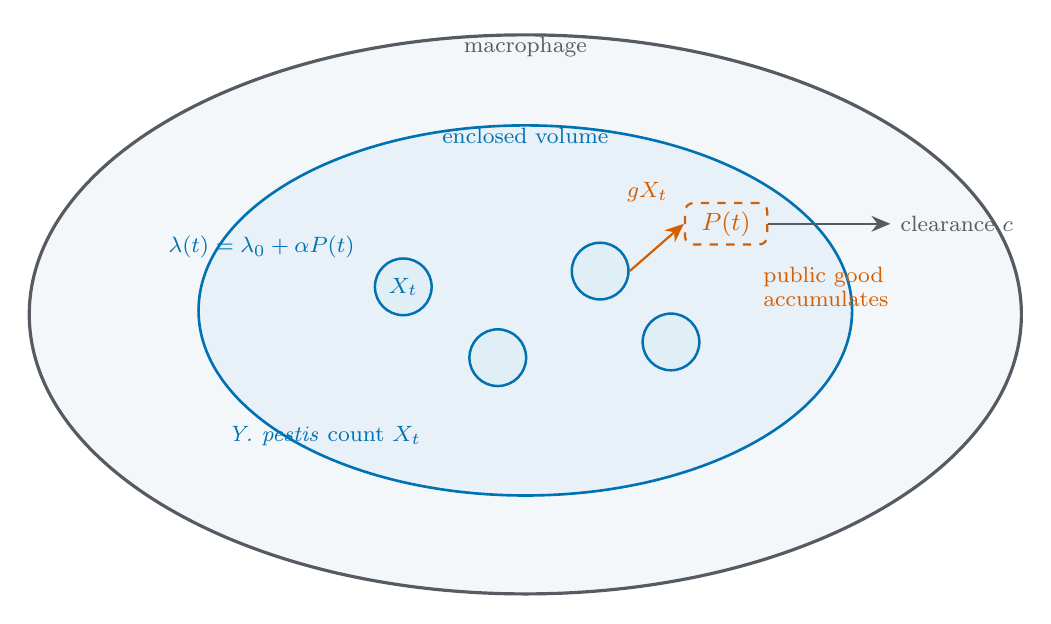
\begin{tikzpicture}[
    >={Stealth[length=2.4mm,width=2.0mm]},
    font=\small,
    bac/.style={circle, minimum size=7.2mm, draw=type1, fill=type1!12,
                line width=0.9pt, font=\footnotesize, text=type1, inner sep=0pt},
  ]

% host-cell outline
\fill[cellfill] (0,0) ellipse (6.3cm and 3.55cm);
\draw[inksoft, line width=1.15pt] (0,0) ellipse (6.3cm and 3.55cm);
\node[font=\footnotesize, text=inksoft, anchor=south] at (0,3.15) {macrophage};

% enclosed volume
\fill[vacfill] (0,0.05) ellipse (4.15cm and 2.35cm);
\draw[type1, line width=0.95pt] (0,0.05) ellipse (4.15cm and 2.35cm);
\node[font=\footnotesize, text=type1, anchor=south] at (0,2.05)
  {enclosed volume};

% bacteria
\node[bac] (x1) at (-1.55,0.35) {$X_t$};
\node[bac] (x2) at (-0.35,-0.55) {};
\node[bac] (x3) at (0.95,0.55) {};
\node[bac] (x4) at (1.85,-0.35) {};
\node[font=\footnotesize, text=type1] at (-2.55,-1.55)
  {\textit{Y.\ pestis} count $X_t$};

% public good label
\node[draw=good, dashed, thick, rounded corners=3pt, inner xsep=6pt,
      inner ysep=3pt, text=good, font=\small] (P) at (2.55,1.15)
  {$P(t)$};
\node[font=\footnotesize, text=good, anchor=west, align=left] at (2.9,0.35)
  {public good\\[-1pt]accumulates};

% production / clearance
\draw[->, good, thick] (x3.east) -- (P.west);
\node[font=\footnotesize, text=good] at (1.55,1.55) {$gX_t$};
\draw[->, inksoft, thick] (P.east) -- ++(1.55,0)
  node[right, font=\footnotesize, text=inksoft, align=left]
  {clearance $c$};

% replication advantage
\node[font=\footnotesize, text=type1, align=center] at (-3.35,0.85)
  {$\lambda(t)=\lambda_0+\alpha P(t)$};

\end{tikzpicture}
\end{document}
